\section{Задание №1} \label{task_01}

\begin{enumerate}
        \item Реализовать генератор схемы Бернулли с заданной вероятностью успеха $p$. На основе генератора схемы Бернулли построить датчик для биномиального распределения.
        \item Реализовать генератор геометрического распределения. Проверить для данного распределения свойство отсутствия памяти.
        \item Рассмотреть игру в орлянку --- бесконечную последовательность испытаний с бросанием правильной монеты. Выигрыш $S_n$ определяется как сумма по всем $n$ испытаниям значений $1$ и $-1$ в зависимости от выпавшей стороны. Проиллюстрировать (в виде ломаной) поведение нормированной суммы $Y(i) = \frac{S_i}{\sqrt{n}}$ как функции от номера испытания $i = 1,\,\ldots,\,n$ для одной отдельно взятой траектории. Дать теоретическую оценку для $Y(n)$ при $n\to\infty$.
\end{enumerate}

\subsection{Задача №1}

\begin{definition}
        \textit{Схемой Бернулли} называется последовательность испытаний, в каждом из которых возможны два исхода~--- <<успех>> и <<неудача>>, при этом <<успех>> в каждом испытании происхоит с одной и той же вероятностью $p \in (0,\,1)$, а <<неудача>>~--- с вероятностью $q \equiv 1 - p$. На испытания в схеме Бернулли налагаются следующие требования: отсутствие взаимного влияния, воспроизводимость, а также сходные~--- но не идентичные~--- условия проведения. 
\end{definition}
\begin{definition}
        Будем говорить, что случайная величина $X$ имеет \textit{распределение Бернулли}, если она принимает всего два значения: 1 и 0 с вероятностями $p$ и $q \equiv 1 - p$ соответственно. Таким образом,
        $$
                \p(X = 1) = p \qquad \mbox{и} \qquad \p(X = 0) = q,
        $$
        то есть событие $\{\,X = 1\,\}$ соответствует <<успеху>>, а $\{\,X = 0\,\}$~---<<неудаче>>. Будем обозначать такую случайную величину
        $$
                X \sim \mbox{Bern}(p).
        $$
\end{definition}

Реализуем генератор схемы Бернулли с заданной вероятностью успеха $p$ следующим образом: пусть нам дана случайная величина $\xi$, равномерно распределённая на отрезке $[0,\,1]$. Тогда случайная величина $X \sim\mbox{Bern}(p)$ задаётся следующим образом:
$$
        X = 
        \I(\xi < p) =
        \begin{cases}
                1, & \mbox{при $0 \leqslant\xi < p$,}\\
                0, & \mbox{при $p\leqslant\xi\leqslant 1$.}
        \end{cases}
$$

\begin{definition}
        Будем говорить, что случайная величина $X$ имеет \textit{биномиальное распределение} с параметрами $n$ и $p$, если
        $$
                \p(X = k) = C_n^kp^k(1-p)^{n-k}, \quad\mbox{где $k\in\N_0$}.
        $$
        В таком случае $X$ интерпретируют как число <<успехов>> в серии из $n$ испытаний схемы Бернулли с вероятностью успеха $p$.
        Будем обозначать такую случайную величину
        $$
                X \sim \mbox{Bi}(n,\,p).
        $$
\end{definition}

Пусть теперь $X\sim\mbox{Bi}(n,\,p)$, а $Y_i \sim \mbox{Bern}(p)$, $i = \overline{1,\,n}$. Тогда, как видно из интерпретации биномиального распределения, датчик биномиальной случайной величины будет иметь вид:
$$
        X = \sum\limits_{i = 1}^{n} Y_i.
$$


\subsection{Задача №2}
\begin{definition}
        Будем говорить, что случайная величина $X$ имеет \textit{геометрическое распределение}, если
        $$
                \p(X = k) =
                (1 - p)^k p =
                q^k p,
                \quad
                \mbox{где $k\in \N_0$}.
        $$
        Геометрически распределенная случайная величина интерпретируется как количество <<неудач>> до первого <<успеха>> в схеме испытаний Бернулли с вероятностью $p$.
        Будем обозначать такие случайные величины
        $$
                X\sim\mbox{Geom}(p).
        $$
        Зная интерпретацию, мы легко строим датчик и для геометрического распределения.
\end{definition}

\begin{assertion}[Свойство отсутствия памяти]
        Пусть $X\sim\mbox{Geom}(p)$, тогда для любых $n,\,m\in\N_0$ справедливо
        $$
                \p(X \geqslant m + n\;|\;X\geqslant m) = \p(X\geqslant n),
        $$
        то есть количество прошлых <<неудач>> не влияет на количество будущих <<неудач>>.
\end{assertion}
\begin{proof}
        Рассмотрим левую часть равенства из условия утверждения:
        \begin{multline*}
                \p(X \geqslant m+n\;|\;X\geqslant m)=
                \frac{\p(X\geqslant m + n,\,X\geqslant m)}{\p(X\geqslant m)}=\\
                =\frac{\p(X\geqslant m+ n)}{\p(X\geqslant m)}=
                \frac{\sum_{i=m+n}^{\infty}q^ip}{\sum_{i=m}^{\infty}q^ip}=
                \frac{q^{m+n}}{q^m}=
                q^n.
        \end{multline*}
        Теперь рассмотрим правую часть равенства:
        $$
                \p(X\geqslant n) = \sum_{i=n}^{\infty}q^ip =
                p\frac{q^n}{1 - q} = q^n.
        $$
        Таким образом, утверждение доказано.
\end{proof}

\subsection{Задача №3}

Рассмотрим игру Орлянка, правила которой описаны в формулировке задания и построим траекторию заданного процесса $Y(i)$.


В данной нормированной сумме $Y$ фигурируют независимые одинаково распределенные случйные величины $X_i$.
Посчитаем их математическое ожидание и дисперсию.

$$
        \E\,X_i = 1 \cdot \frac12 - 1 \cdot \frac12 = 0,
$$
$$
        \Var\,X_i = \frac12 \cdot (1 - 0)^2 + \frac12 \cdot (-1 - 0)^2 = \frac14.
$$
Теперь можем воспользоваться следующей теоремой.
\begin{theorem}[Центральная предельная теорема]
        Пусть $X_1,\,\ldots,\,X_n,\,\ldots$ есть бесконечная последовательность независимых одинаково распределенных случайных величин, имеющих конечное математическое ожидание $\mu$ и дисперсию $\sigma^2$. Пусть также $S_n = \sum_{i=1}^{n} X_i$. Тогда
        $$
                \frac{S_n - \mu n}{\sigma\sqrt{n}} \longrightarrow \mbox{N}(0,\, 1)
        $$
        по распределению при $n\to\infty$.
\end{theorem}
Получается, что
$$
        2\lim\limits_{n\to\infty}Y(n) \xrightarrow{dist.} N(0,\,1).
$$
Для оценки этого значения воспользуемся <<правилом трёх сигм>>.
\begin{theorem}
        Практически все значения нормально распределённой случайной величины $\xi \sim N(\mu,\,\sigma^2)$ лежат в интервале $(\mu - 3\sigma,\,\mu + 3\sigma)$. Более строго~--- приблизительно с вероятностью $0,9973$ значение нормально распределённой случайной величины лежит в указанном интервале.
\end{theorem}
Таким образом, приблизительно с вероятностью $0,9973$
$$
        -\frac32\leqslant\lim\limits_{n\to\infty}Y(n)\leqslant\frac32.
$$

\clearpage
\begin{figure}[t]
        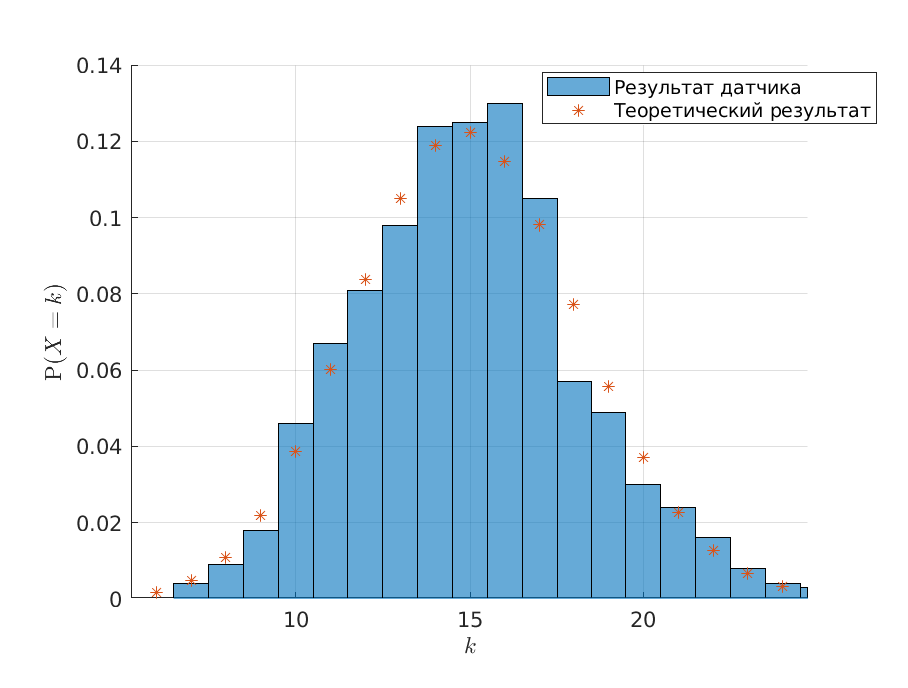
\includegraphics[width=0.5\linewidth]{task_01/bi1000.eps}
        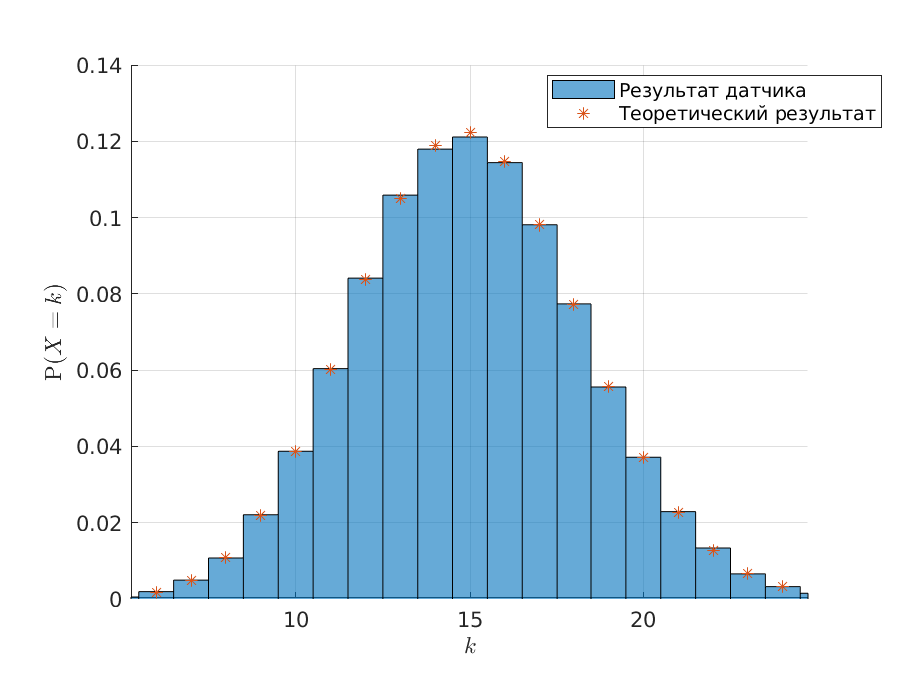
\includegraphics[width=0.5\linewidth]{task_01/bi100000.eps}
        \caption{Гистограмма биномиального распределения случайной величины с параметрами $n = 50$, $p = \frac{3}{10}$ при $10^3$~(слева) и $10^5$~(справа) испытаний.}
\end{figure}
\begin{figure}[b]
        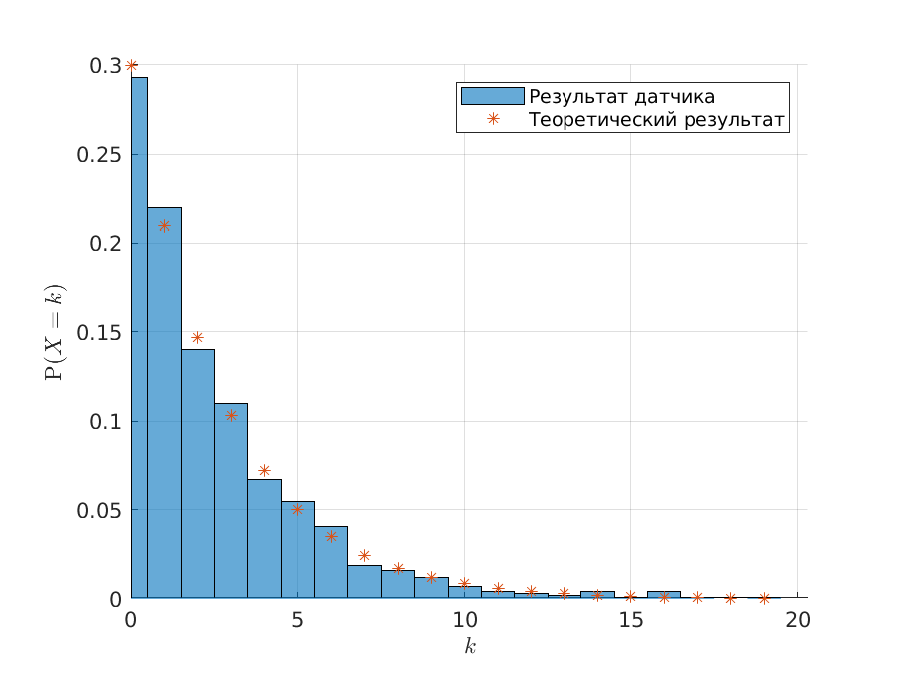
\includegraphics[width=0.5\linewidth]{task_01/geom1000.eps}
        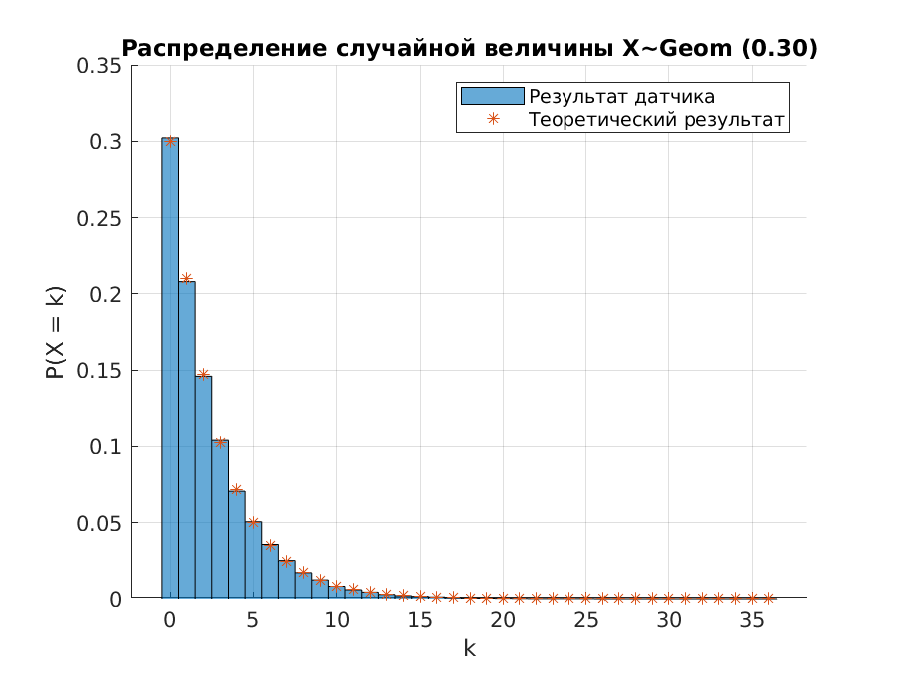
\includegraphics[width=0.5\linewidth]{task_01/geom100000.eps}
        \caption{Гистограмма геометрического распределения случайной величины с параметром $p = \frac{3}{10}$ при $10^3$~(слева) и $10^5$~(справа) испытаний.}
\end{figure}
\begin{figure}[h]
        \noindent
        \centering
        {
                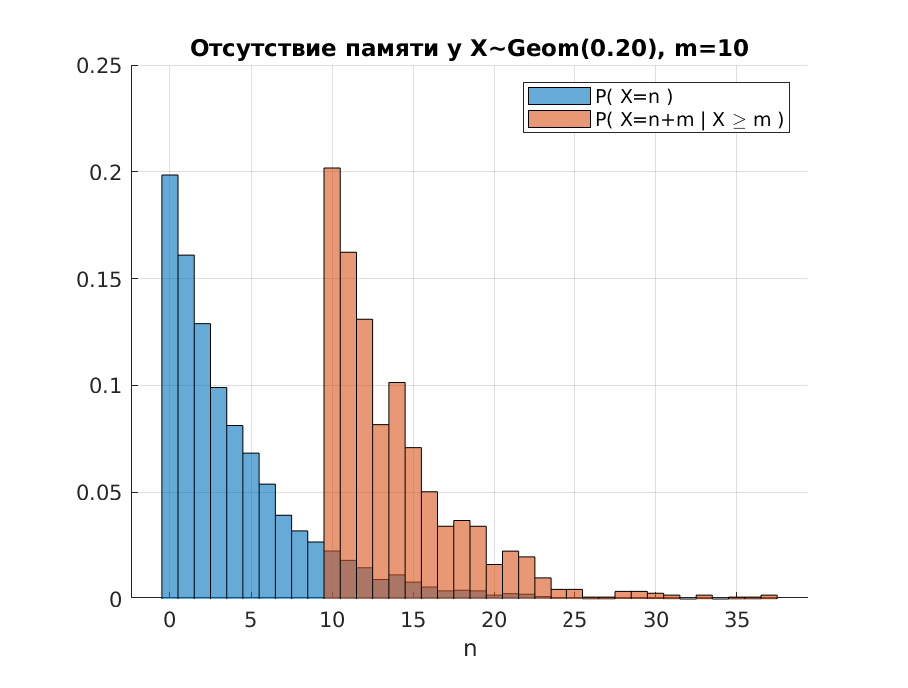
\includegraphics[width=120mm]{task_01/memory.eps}
        }
        \caption{Гистограмма геометрического распределения, демонстрирующая его свойство отсутствия памяти. Здесь задан параметр геометрического распределения $p = \frac{2}{10}$, а также <<сдвиг>> $m = 10$.}
\end{figure}
\begin{figure}[h]
        \noindent
        \centering
        {
                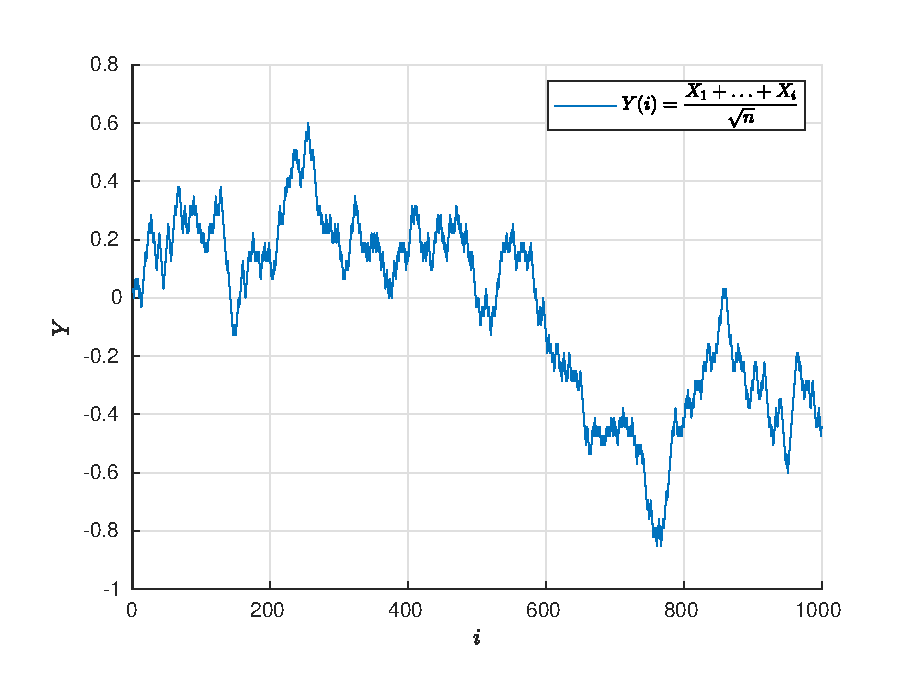
\includegraphics[width=120mm]{task_01/orl.eps}
        }
        \caption{Иллюстрация варианта поведения нормированной суммы $Y(i)$ игры в орлянку на отрезке $1 \leqslant i\leqslant 10^3$.}
\end{figure}